\documentclass{patmorin}
\listfiles
\usepackage{pat}
\usepackage{paralist}
\usepackage{dsfont}  % for \mathds{A}
\usepackage[utf8x]{inputenc}
\usepackage{skull}
\usepackage{paralist}
\usepackage{graphicx}
\usepackage[noend]{algorithmic}
\usepackage{bbm}  % needed for \mathbbm{1}

\usepackage[normalem]{ulem}
\usepackage{cancel}
%\usepackage{enumitem}

\usepackage{todonotes}

% etoolbox allows for robust commands that don't need \protect, e.g.
% \newrobustcmd{\onesub}{\mathord{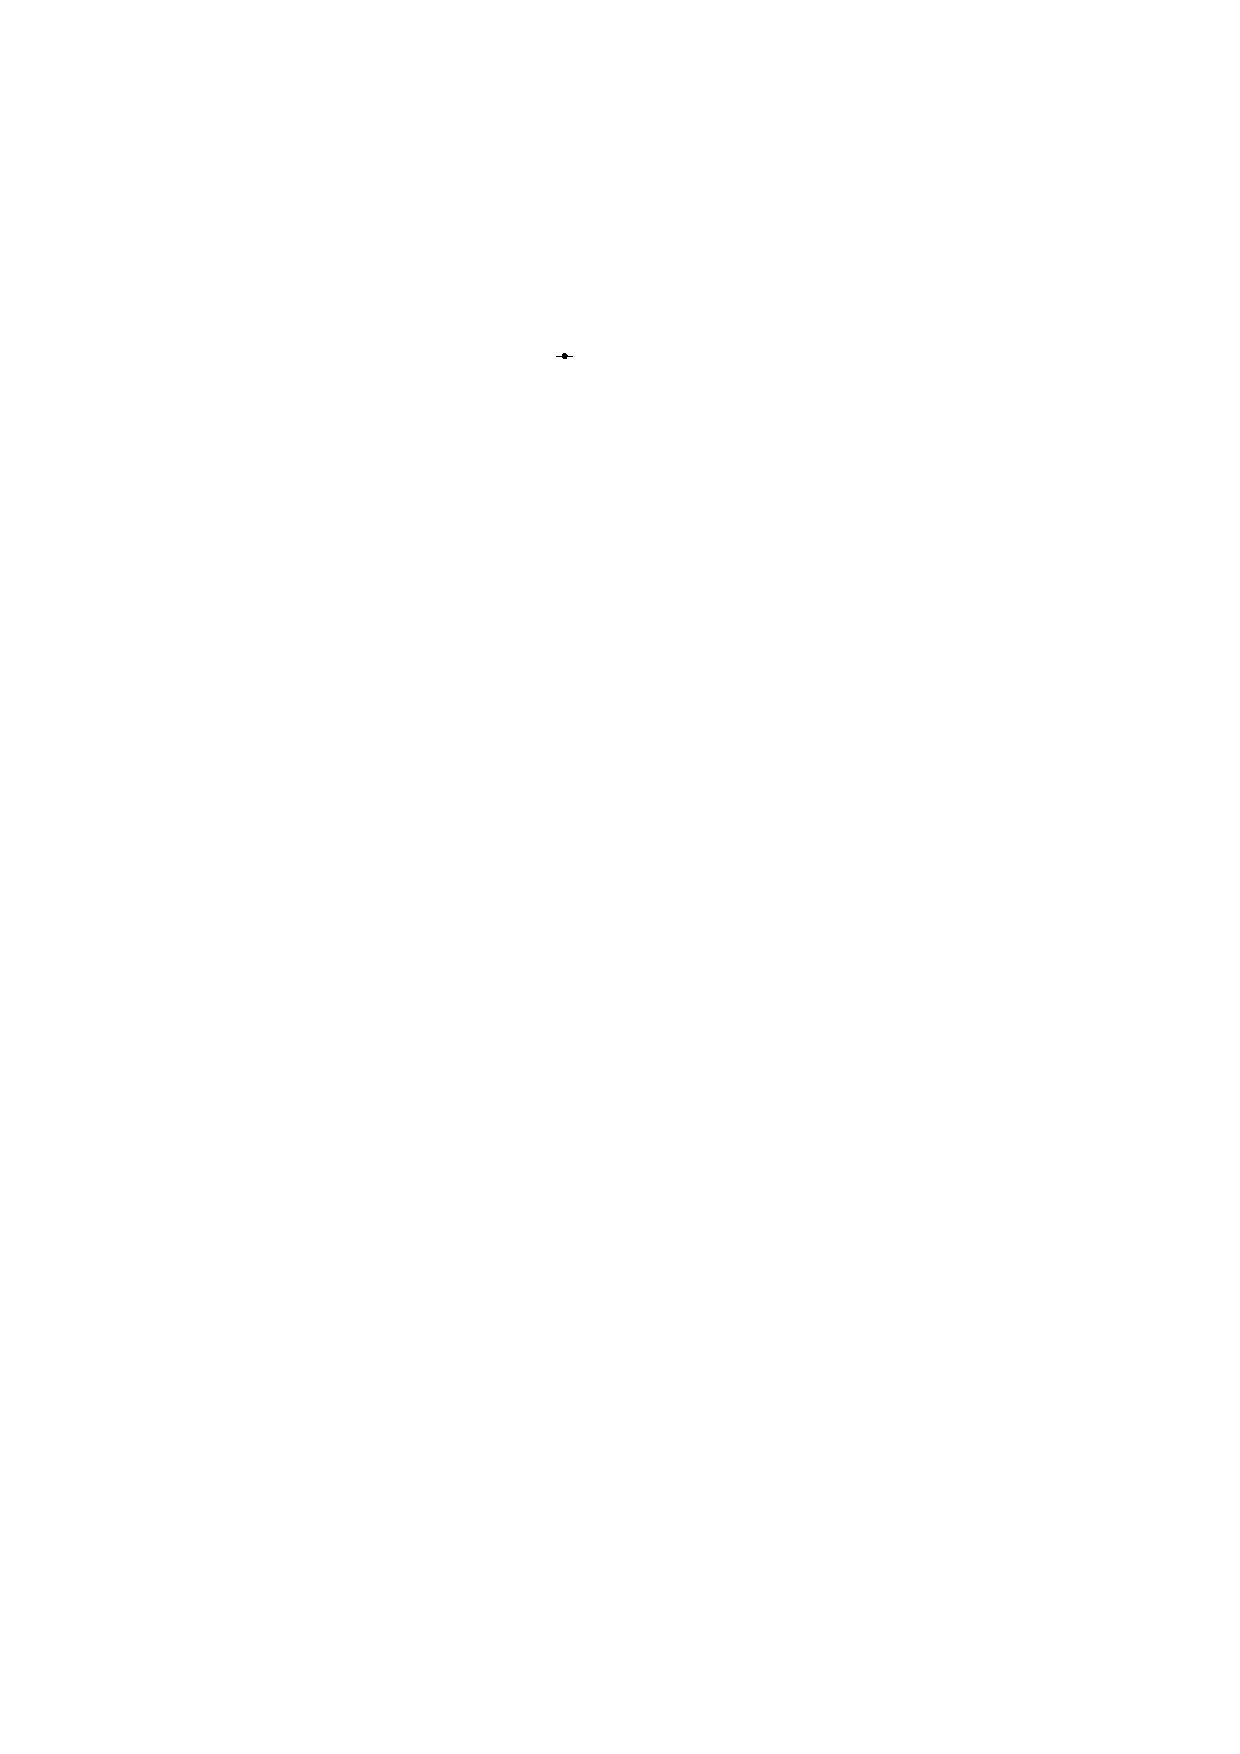
\includegraphics{figs/one-sub}}}
% \subsection{Approximate Voronoi Diagrams in $G^{\onesub}_k$}
\usepackage{etoolbox}

\usepackage[longnamesfirst,numbers,sort&compress]{natbib}

\usepackage[mathlines]{lineno}
\setlength{\linenumbersep}{2em}
% \linenumbers
% \rightlinenumbers
% \linenumbers
\newcommand*\patchAmsMathEnvironmentForLineno[1]{%
 \expandafter\let\csname old#1\expandafter\endcsname\csname #1\endcsname
 \expandafter\let\csname oldend#1\expandafter\endcsname\csname end#1\endcsname
 \renewenvironment{#1}%
    {\linenomath\csname old#1\endcsname}%
    {\csname oldend#1\endcsname\endlinenomath}}%
\newcommand*\patchBothAmsMathEnvironmentsForLineno[1]{%
 \patchAmsMathEnvironmentForLineno{#1}%
 \patchAmsMathEnvironmentForLineno{#1*}}%
\AtBeginDocument{%
\patchBothAmsMathEnvironmentsForLineno{equation}%
\patchBothAmsMathEnvironmentsForLineno{align}%
\patchBothAmsMathEnvironmentsForLineno{flalign}%
\patchBothAmsMathEnvironmentsForLineno{alignat}%
\patchBothAmsMathEnvironmentsForLineno{gather}%
\patchBothAmsMathEnvironmentsForLineno{multline}%
}


% Taken from
% https://tex.stackexchange.com/questions/42726/align-but-show-one-equation-number-at-the-end
\newcommand\numberthis{\addtocounter{equation}{1}\tag{\theequation}}

\newcommand{\defin}[1]{\emph{\color{brown}#1}}
\setlength{\parskip}{1ex}

% Document-specific commands and math operators
\DeclareMathOperator{\tw}{tw}
\DeclareMathOperator{\td}{td}
\DeclareMathOperator{\chicen}{\chi_{\mathrm{cen}}}
\DeclareMathOperator{\chilin}{\chi_{\mathrm{lin}}}
\DeclareMathOperator{\dist}{dist}
\DeclareMathOperator{\vor}{Vor}

\DeclareMathOperator{\binomial}{binomial}

\newrobustcmd{\onesub}{\mathord{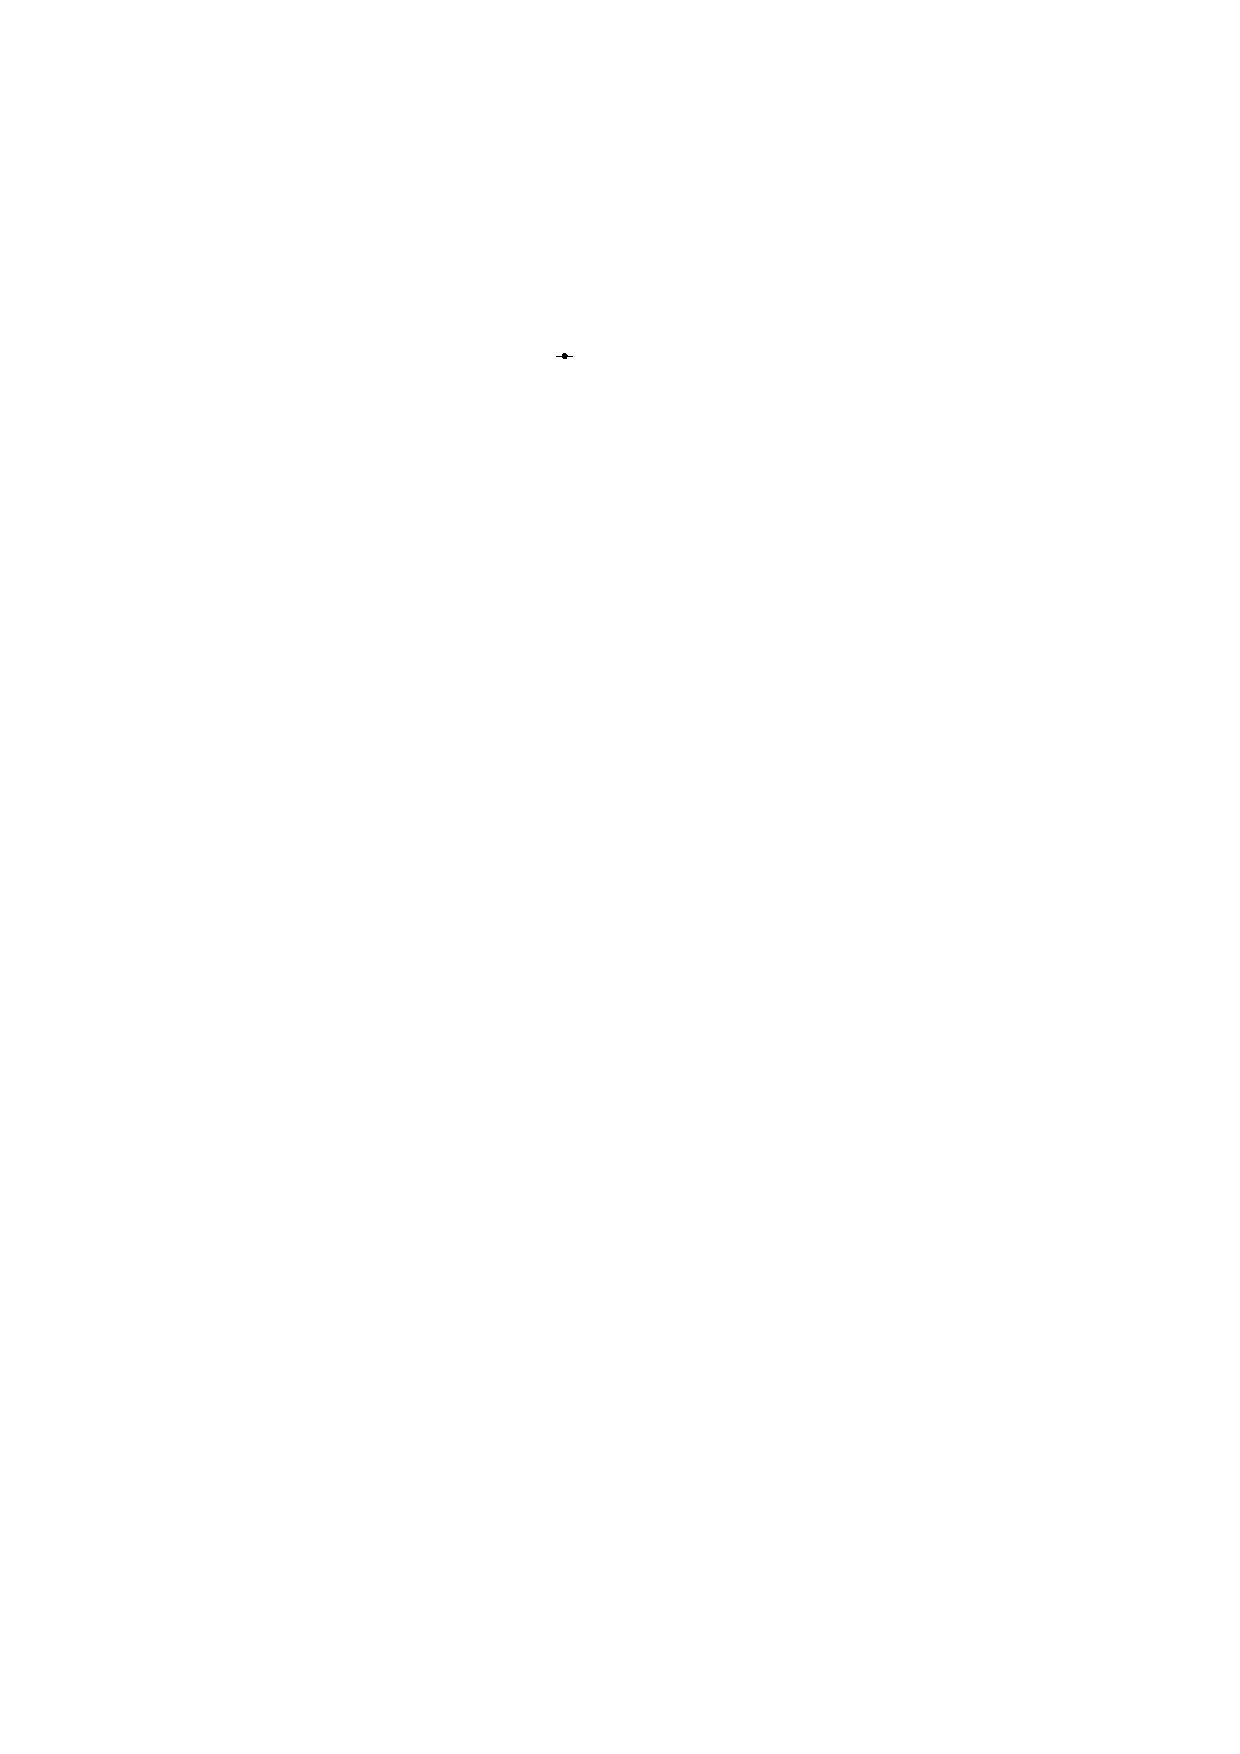
\includegraphics{figs/one-sub}}}
\newrobustcmd{\leftup}{\mathord{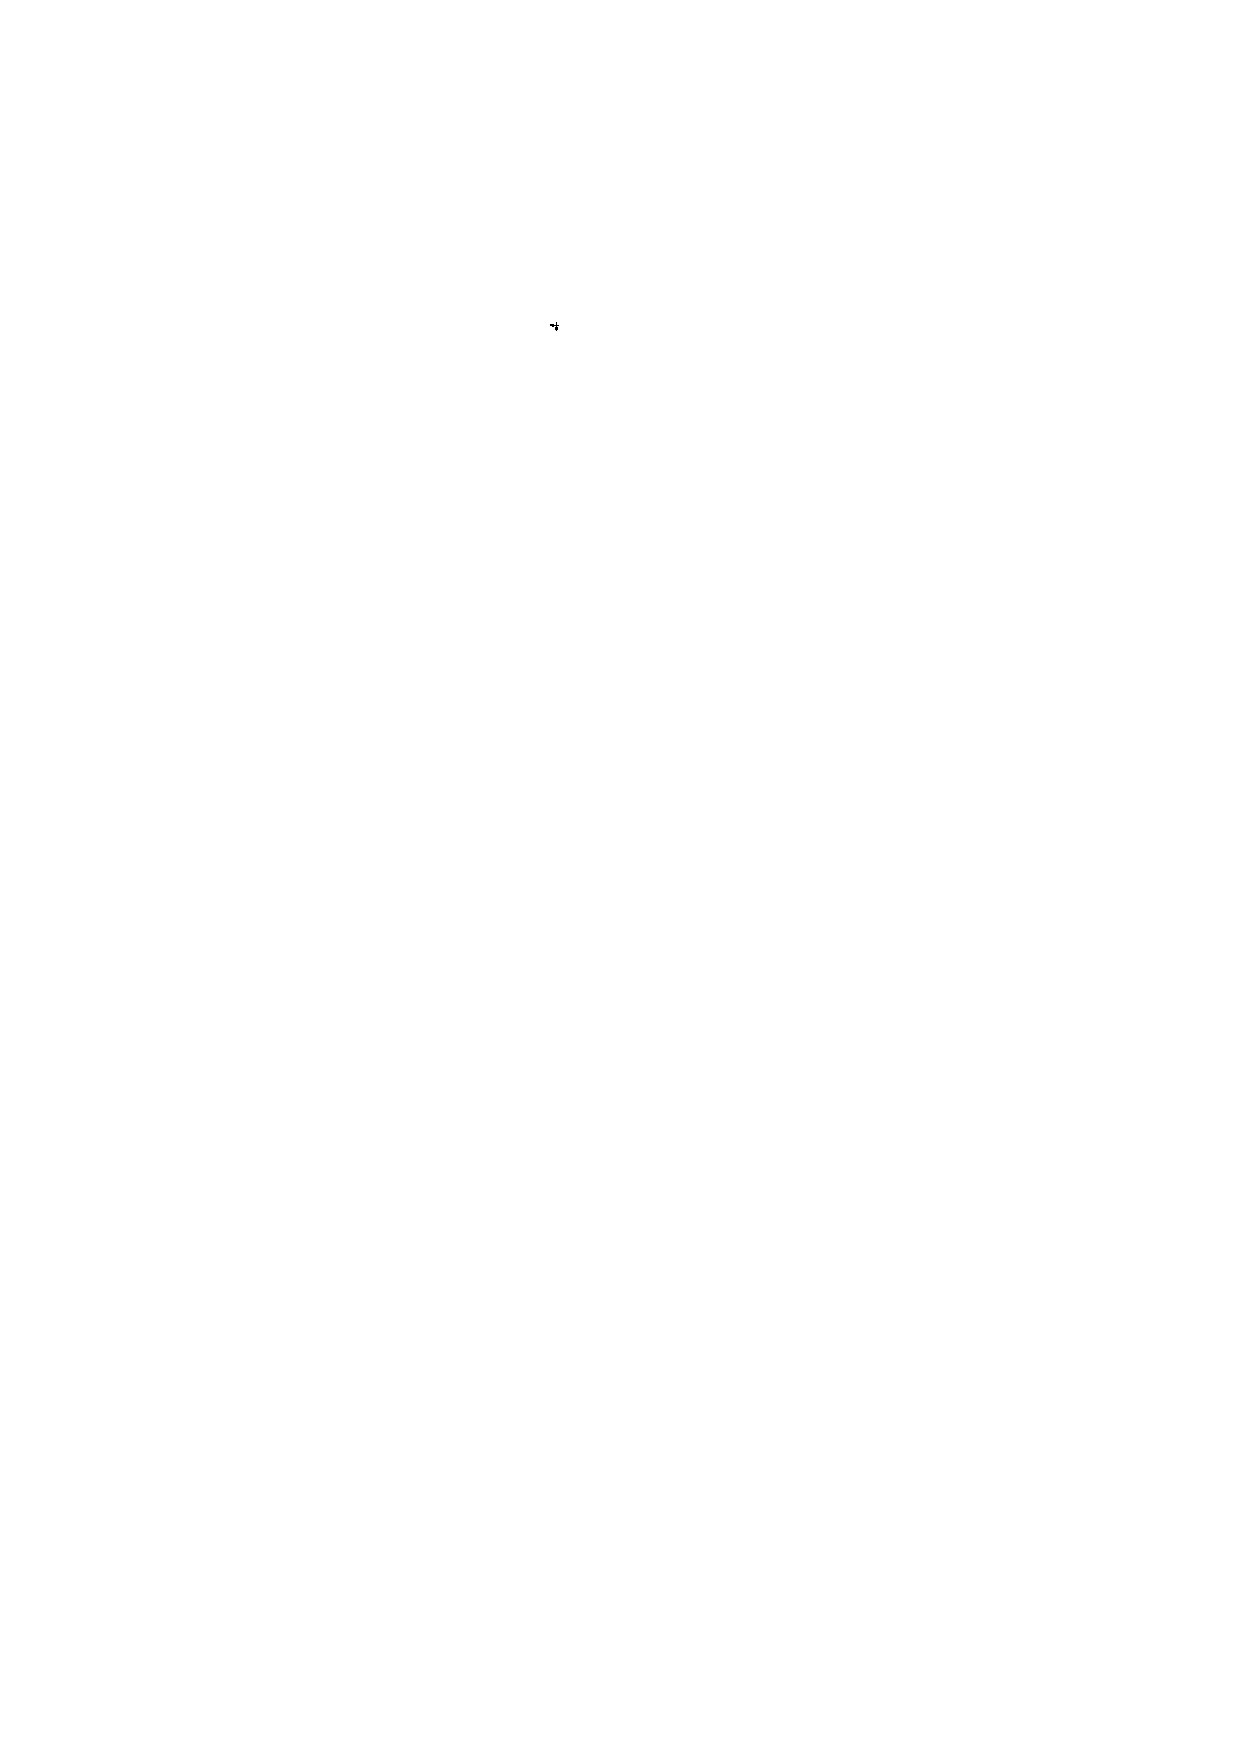
\includegraphics{figs/left-up}}}

\title{\MakeUppercase{Linear versus centred Colouring Numbers}\thanks{This research was partly funded by NSERC.}}
\author{Prosenjit~Bose, Vida~Dujmović, Hussein~Houdrouge, Mehrnoosh~Javarsineh, and Pat~Morin}

\DeclareMathOperator{\VE}{\mathit{VE}}

\date{}


\begin{document}

\maketitle
\renewcommand{\E}{\mathbb{E}}
\renewcommand{\Pr}{\mathbb{P}}

\begin{abstract}
    These are some notes on the relationships betwee linear colouring numbers and centred colouring numbers.
\end{abstract}

\section{Introduction}

Let $G$ be a simple undirected graph.  A \emph{$k$-colouring} of $G$ is any function $\varphi:V(G)\to S$ where $S$ is a set of size $k$.  A vertex $v$ of $G$ is a \emph{centre} of $G$ with respect to $\varphi$ if $\varphi(v)\not\in\{\varphi(w):w\in V(G)\setminus\{v\}\}$, i.e., $v$ is the unique vertex of $G$ having colour $\varphi(v)$.  A colouring $\varphi$ of $G$ is \emph{centred} if every connected subgraph of $G$ has a centre with respect to $\varphi$. A colouring $\varphi$ of $G$ is \emph{linear} if every simple path in $G$ has a centre with respect to $\varphi$.

The \emph{centred chromatic number} $\chicen(G)$ of $G$ is the minimum integer $c$ such that $G$ has a centred $c$-colouring.  We note that an easy argument shows that centered chromatic number and treedepth are equivalent, i.e., $\td(G)=\chicen(G)$ for every graph $G$. The \emph{linear chromatic number} of $G$ is the minimum integer $\ell$ such that $G$ has a linear $\ell$-colouring.  Since every path in $G$ is a connected subgraph of $G$, every centred colouring of $G$ is also a linear colouring of $G$, so $\chilin(G)\le\chicen(G)$.

The question of upper bounding $\chicen(G)$ by some function of $\chilin(G)$ was considered by \citet[Theorem~1]{kun.obrien.ea:polynomial} who showed the following result:

\begin{thm}[\citet{kun.obrien.ea:polynomial}]\label{kun_obrien_general}
  For any graph $G$, $\chicen(G)\le \chilin^{190}(G)\cdot\log^{O(1)}(\chilin(G))$.\todo{Update with most recent numbers}
\end{thm}


Their proof of \cref{kun_obrien_general} has three steps:
\begin{enumerate}
  \item A theorem of \citet{kawarabayashi.rossman:polynomial} shows that, if $\chicen(G)\ge k^{190}\log^{O(1)} k$ then $\chilin(G)\ge k^{38}$ or $G$ has treewidth $\tw(G)\ge k^{38}$.  In the former case there is nothing left to prove.
  \item The current-best version of the Excluded Grid Theorem due to \citet{chuzhoy:improved} shows that, if $\tw(G)\ge k^{38}$, then $G$ contains an $\Omega(k^2\times k^2)$ grid minor.
  \item A technical lemma \cite[Lemma~5]{kun.obrien.ea:polynomial} shows that, if $G$ contains a $k^2\times k^2$ grid minor, then $\chilin(G)\in\Omega(k)$.
\end{enumerate}

These notes are an attempt to improve the bound in \cref{kun_obrien_general} in the general case as well as for some special classes of graphs. First we point out that some new results can already reduce the exponent from $190$ to $39$ and eliminate the polylog factor.  (These improvements are already described by \citet[Theorem~1.9]{czerwinski.nadara.ea:improved}.)

First, \citet{chuzhoy.tan:towards} improved the exponent in the Excluded Grid Theorem:  There exists a constant $c$ such that any graph $G$ with $\tw(G)\ge k^{18}\log^c k$ has a $k\times k$ grid minor.  This already improves the bound from $k^{190}$ to $k^{90}$.
Next, a recent result of \citet[Theorem~1.4]{czerwinski.nadara.ea:improved} shows that if $b$ is the maximum treedepth of any tree contained in $G$ then $\td(G)\le b\cdot\tw(G)$ (and the proof is easy).  Therefore, if $\td(G)\ge k^{19}$ then at least one of the following cases applies:
\begin{enumerate}
    \item $\tw(G)\ge k^{18}$: In this case the proof follows Steps~2 and 3 as before, but using the grid minor result of \citet{chuzhoy.tan:towards} to show that $\chilin(G)\in\Omega(k)$.
    \item $G$ contains a tree $T$ of treedepth $k$.  The same paper \cite[Lemma~1.6]{czerwinski.nadara.ea:improved} shows that any tree $T$ of treedepth $k$ contains a subcubic subtree of treedepth $\Omega(k)$.
    A theorem of \citet{kun.obrien.ea:polynomial} shows that, for any subcubic tree $T$, $\chicen(T) \le (\log_2 3)\cdot\chilin(T)$.  Therefore, in this case $\chilin(G)\ge\chilin(T)\ge \chicen(T)/\log_2 3 = \Omega(k)$.
\end{enumerate}

This gives the following improvement to \cref{kun_obrien_general}
\begin{thm}[\citet{czerwinski.nadara.ea:improved}]\label{kun_obrien_general2}
  For any graph $G$, $\chicen(G)\in O(\chilin^{19}(G))$.
\end{thm}



As a next step, we would like to improve the third part of the argument to show that, if $G$ contains a $k\times k$ grid minor, then $\chilin(G)\in \Omega(k)$.  This, by itself, would reduce the exponent in \cref{kun_obrien_general2} from $39$ to $20$.  We observe that the first two parts of the argument are both ``heavy hammers'' and that, for some special graph classes, much lighter hammers suffice.  For example, if we consider only planar graphs, then it is well known that any planar graph $G$ of treewidth $k$ contains an $\Omega(k\times k)$ grid minor.  This already reduces the exponent in \cref{kun_obrien_general2} further (for planar graphs) to $3$ ($2$ if we can prove the result for grid minors).  If one could prove a similar result for the first ``heavy hammer'' then this would show that, for any planar graph $G$, $\chicen(G)\in O(\chilin(G))$.


\section{Preliminaries}

% For a graph $G$ and a vertex $v\in V(G)$, $\deg_G(v):=|\{vw\in E(G)\}|$ denotes the degree of $v$ in $G$.  For a any $S\subseteq V(G)$, $\deg_G(S):=\sum_{v\in S}\deg_G(v)$ is the total degree of $S$.

% For a vertex $v$ in a graph $G$, the \emph{open neighbourhood} of $v$ is $N_G(v):=\{w:vw\in E(G)\}$ and the \emph{closed neighbourhood} of $v$ is $N_G[v]:=\{v\}\cup N_G(v)$.  For any $S\subseteq V(G)$, $N_G(s):=\bigcup_{v\in S}N_G(v)$ and $N_G[s]:=\bigcup_{v\in S}N_G[v]$.  The subgraph $G[S]$ of $G$ \emph{induced} by $S$ is the graph with vertex set $V(G[S]):=S\cap V(G)$ and edge set $E(G[S]):=\{vw\in E(G):\{v,w\}\subseteq S\}$.

In this paper, all graphs are simple and undirected. For a graph $G$, $V(G)$ denotes the vertex set of $G$, $E(G)$ denotes the edge set of $G$ and $\VE(G):=V(G)\cup E(G)$.

% For a graph $G$ and a partition $\mathcal{P}$ of $V(G)$, the \emph{quotient graph} $G/\mathcal{P}$ is the graph with vertex set $\mathcal{P}$ and that contains an edge $vw$ if and only $G$ contains an edge with one endpoint in $v$ and one endpoint in $w$.  When $\mathcal{P}$ consists of disjoint subsets of $V(G)$ that do not necessarily cover $V(G)$ then we use the convention that $G/\mathcal{P}:=G/\mathcal{P'}$ where $\mathcal{P}'$ is the completion of $\mathcal{P}$ obtained by introducing each missing element of $V(G)$ as singleton set.  More precisely $\mathcal{P'}:=\mathcal{P}\cup\{\{v\}:v\in V(G)\setminus(\cup P)\}$.


% A \emph{subdivision} of a graph $G$ is any graph $G'$ that can be obtained from $G$ by replacing each edge $vw$ of $G$ with a path $v,s_1,s_2,\ldots,s_\ell,w$ in which each of the (newly introduced) internal vertices $s_1,\ldots,s_\ell$ have degree exactly $2$.  Each vertex in $V(G')\setminus V(G)$ is called a \emph{subdivision vertex}.  A $\ell$-subdivision of $G$ is a subdivision of $G$ in which each edge of $G$ is replaced by a path that has exactly $\ell$ internal vertices.  For any graph $G$, we use $G^{\onesub}$ to denote the $1$-subdivision of $G$.  Note that there is a natural bijection between the vertex set $V(G^{\onesub})$ and the vertex/edge set $V(G)\cup E(G)$.  A $\le\!\!\ell$-subdivision of $G$ is a subdivision of $G$ in which each edge of $G$ is replaced by a path that has at most $\ell$ internal vertices.


We make use of the following (polygamous) generalisation of Hall's Marriage Theorem, which follows from Hall's Marriage Theorem by replacing each vertex $x\in X$ with a $d$-tuple $x_1,\ldots,x_d$ each having the same neighbours as $x$.

% \begin{lem}\label{normal_hall}
%   Let $G$ be a bipartite graph with parts $X$ and $Y$ such that, for any $A\subseteq X$, $|N_G(A)|\ge |A|+1$.  Then $G$ contains a subgraph $M$ (a matching) such that $\deg_M(x)=1$ for each $x\in X$ and $\deg_M(y)\le 1$ for each $y\in Y$.
% \end{lem}


\begin{cor}\label{d_hall}
  Let $d\ge 1$ be an integer and let $G$ be a bipartite graph with parts $X$ and $Y$ such that, for any $A\subseteq X$, $|N_G(A)|\ge d|A|$.  Then $G$ contains a subgraph $M$ such that $\deg_M(x)=d$ for each $x\in X$ and $\deg_M(y)\le 1$ for each $y\in Y$.
\end{cor}


\begin{lem}\label{weighted_lovasz}
  Let $E:=\{E_1,\ldots,E_n\}$ be a set of events in some probability space $(\Omega,\Pr)$.  For each $i\in\{1,\ldots,n\}$, let $\Gamma_i\subseteq E$ be such that the event $E_i$ is mutually independent of $\Gamma_i$,\footnote{An event $A$ is mutually independent of a set $\{B_1,\ldots,B_r\}$ of events if, for any disjoint sets $I,J\subseteq\{1,\ldots,r\}$, $\Pr(A\cap\bigcap_{i\in I} B_i\cap\bigcap_{j\in J} \overline{B}_j=\Pr(A)\Pr(\bigcap_{i\in I} B_i\cap\bigcap_{j\in J} \overline{B}_j)$.} and let $w:E\to(0,1)$ be such that
  \[
      \Pr(E_i) \le w(E_i)\cdot\prod_{E_j\in\Gamma_i}(1-w(E_j))  \enspace .
  \]
  Then $\Pr(\overline{E_1}\cap\cdots\cap\overline{E_n}) > 0$.
\end{lem}

% \begin{proof}
%   \todo[inline]{Surely this is known}
% \end{proof}
%
%
% \todo[inline]{Surely this next lemma is well-known?}
% We make use of the following generalization of Hall's Marriage Theorem \cite{hall:on}:
% \begin{lem}\label{hall_vees}
%   Let $G$ be a bipartite graph with vertex parts $A$ and $B$ and having the property that, for any $A_0\subseteq A$, $|N_G(W)|\ge 2|A_0|$.  Then $G$ contains a subgraph $\Lambda$ in which each vertex of $A$ has degree exactly two and each vertex of $B$ has degree at most one.
% \end{lem}
%
% \begin{proof}
%   Let $\Lambda$ be a subgraph of $G$ in which each vertex of $A$ has degree at most two, each vertex of $B$ has degree at most one, and that maximizes $\deg_\Lambda(A)$.  If $\deg_{\Lambda}(A) = 2|\Lambda|$ then there is nothing to prove. Assume therefore, for the sake of contradiction,  that there exists $v_0\in A$ with $\deg_\Lambda(v_0) < 2$.
%
%   We say that a path $v_0,\ldots,v_m$ in $G$ is \emph{$\Lambda$-aternating} if $v_iv_{i+1}\in E(\Lambda)$ for all odd $i\in\{0,\ldots,m-1\}$ and $v_iv_{i+1}\not\in E(\Lambda)$ for all even $i\in\{0,\ldots,m\}$.  Observe that any such path has even length so that it ends at a vertex $v_m\in A$.  Otherwise, replacing the edges $\lfloor m/2\rfloor$ edges $\{v_1v_2,v_3v_4,\ldots,v_{m-2}v_{m-1}\}\in E(\Lambda)$ with the $\lceil m/2\rceil$ edges $\{v_0v_1,v_2v_3,\ldots,v_{m-1}v_m\}$ does not change $\deg_\Lambda(v)$ for any $v\in A_0\setminus\{v_0\}$ but does increase  $\deg_\Lambda(v_0)$, contradicting the assumption that $\Lambda$ maximizes $\deg_\Lambda(A)$.
%
%   Let $A_0\subseteq A$ and $B_0\subseteq B$ be the subsets of $A$ and $B$, respectively, that can be reached from $v_0$ by $\Lambda$-alternating paths.
%   Observe that, for any $x\in B_0$,  there is exactly one edge $vx$ of $\Lambda$ incident on $x$ and the other endpoint $v$ of this edge is in $A_0$.  Let $a$ be the number of edges of $\Lambda$ having one endpoint $A_0$ and one endpoint in $B_0$, so that $a=\deg_\Lambda(B_0)=|B_0|$.  Let $b$ be the number of edges of $\Lambda$ having one endpoint in $A_0$ and one endpoint in $B\setminus B_0$, so that $\deg_\Lambda(A_0)=a+b = |B_0|+b$.    Since $\deg_{\Lambda}(v) \le 2$ for each $v\in A_0$ and $\deg_\Lambda(v_0)<2$, $\deg_\Lambda(A_0)<2|A_0|$.  This yields the desired contradiction, since $|N_\Lambda(A_0)| \le \deg_\Lambda(A_0) = |B_0|+b = \deg_\Lambda(A_0)< 2|A_0|$.greater than
% \end{proof}
%
% \begin{rem}
%   The constant $2$ that appears twice in \cref{hall_vees} can be replaced with any positive integer $c$.
% \end{rem}


\section{The Linear Colouring Number of Pseudogrids}

% Refer to \cref{grid_figure}.
For positive integers $a$ and $b$, the \emph{$a\times b$ grid} $G_{a\times b}$ is the graph with vertex set $V(G_{a\times b}):=\{1,\ldots,a\}\times\{1,\ldots,b\}$ and that contain an edge with endpoints $(v,w)$ and $(x,y)$ if and only if $|v-x|+|w-y|=1$.  For each $i\in\{1,\ldots,a\}$, the \emph{$i$th column} of $G_{a\times b}$ is the vertex set $\{(i,1),\ldots,(i,b)\}$ and, for each $j\in\{1,\ldots,b\}$, the $j$th row is the vertex set $\{(1,j),\ldots,(a,j)\}$.

In this work, we need to work with pseudogrids.  An \defin{$a\times b$-pseudogrid} is any graph that can be obtained from $G_{a\times b}$ in the following way:
\begin{compactenum}
  \item Replace each edge $vw$ of $G_{a\times b}$ with a path $\overline{P}_{vw}$ whose endpoints are $v$ and $w$.  (In other words, $\overline{P}_{vw}$ is a path obtained by subdividing the edge $vw$ zero or more times.)
  \item Replace each degree-$4$ vertex $(x,y)$ of $G_{a\times b}$ with a path $P_v$. If $P_v$ has only one vertex then this operation has no effect.  Otherwise, $P_v$ has two endpoints $p$ and $q$ and
  \begin{compactenum}[(Q1)]
    \item \label{q_i} $p$ is adjacent to $\{(x-1,y), (x,y-1)\}$ and $q$ is adjacent to $(x+1,y),(x,y+1)$;
    \item \label{q_ii} $p$ is adjacent to $\{(x,y+1), (x-1,y)\}$ and $q$ is adjacent to $(x,y-1),(x+1,y)$; or
    \item \label{q_iii} $p$ is adjacent to $\{(x-1,y),(x+1,y)\}$ and $q$ is adjacent to $\{(x,y-1),(x,y+1)\}$.
  \end{compactenum}
\end{compactenum}

Let $G$ be an $a\times b$ pseudogrid.  For an edge $vw$ of $G_{a\times b}$, we let $P_{vw}:=\overline{P}_{vw}-\{v,w\}$ denote the (possibly empty) subpath containing the internal vertices of $\overline{P}_{vw}$.  For each vertex $v$ of $G_{a\times b}$ of degree less than $4$ we define $P_{v}$ to be the $1$-vertex path that contains only $v$.  In this way, $\mathcal{P}:=\{V(P_\mu):\mu\in \VE(G_{a\times b})\}$ is a partition of $V(G)$ into induced paths.  We call $\mathcal{P}$ the \defin{grid-partition} of $G$.
% and we denote it by $(P_\mu:\mu\in \VE(G_{a\times b}))$.
% This defines a mapping $\delta:V(G)\to V(G_{a\times b})\cup E(G_{a\times b})$ where $u\in V(P_{\delta(u)})$ for each $u\in v(G)$.

% Then each vertex $u$ of $G$ naturally corresponds to an edge or vertex $u'$ of $G_{a\times b}$:  If $u$ is a vertex of $P_{vw}$ then $u'=vw$; if $u$ a vertex of $P_v$ then $u'=v$; and otherwise $u'=u$.  This latter case occurs precisely when $u'$ is one of the boundary vertices of $G_{a\times b}$.

Each row $R':=v_1,\ldots,v_a$ of $G_{a\times b}$ corresponds naturally to a path $R$ of $G$. The path $R$ contains $V(\overline{P}_{v_iv_{i+1}})$ for each $i\in\{1,\ldots,a-1\}$.  However, for $i\in\{2,\ldots,a-1\}$ $R$ may or may not contain $V(P_{v_i})$.  In particular, if $P_{v_i}$ was created using (Q\ref{q_iii})\todo{Fix this!} then $R$ does not contain any internal vertices in $P_{v_i}$.
Similarly, a column $C':=v_1,\ldots,v_b$ of $G_{a\times b}$ corresponds to a path that contains $V(\overline{P}_{v_jv_{j+1}})$ for each $j\in\{1,\ldots,b-1\}$. This correspondence allows us to talk about the rows and columns of $G$, which we will do next.

As part of our proof, we use the operation of \defin{deleting} a row (or column) $R$ of $G$, which works as follows:  We remove all edges of $R$ from $G$ and eliminate any isolated vertices.  If this produces vertices of degree $1$ (which happens when $R$ is the first or last row of $G$ or when $R=v_1,\ldots,v_a$ does not contains $P_{v_i}$ for some $i\in\{1,\ldots,r\}$) then we repeatedly remove degree-$1$ vertices until none remain.  If $G$ is an $a\times b$ pseudogrid and we delete some row $R$, then the resulting graph is an $a\times (b-1)$ pseudogrid.  Similarly, if we delete column $C$ of $G$, then the resulting graph is an $(a-1)\times b$ pseudogrid.


\subsection{Pseudogrids with Exclusively Frequent Colours}

For convenience, let $G_k:=G_{k\times k}$.
Let $G$ be a $k\times k$ pseudogrid with grid partition $\mathcal{P}:=(P_\mu:\mu\in\VE(G_{k}))$ and let $\varphi:V(G)\to\{1,\ldots,c\}$ be a vertex colouring of $G$.  For any $\mu\in\VE(G_{k})$, we let $\varphi_{\mathcal{P}}(\mu):=\{\varphi(v):v\in V(P_\mu)\}$.  For any colour $\alpha\in\{1,\ldots,c\}$, define $\varphi^{-1}(\alpha):=\{v\in V(G):\varphi(v)=\alpha\}$ and define $\varphi_\mathcal{P}^{-1}(\alpha):=\{\mu\in \VE(G_{k\times k}):\alpha\in\varphi_\mathcal{P}(\mu)\}$.  For any colour set $A\subseteq\{1,\ldots,c\}$ define $\varphi^{-1}(A):=\bigcup_{\alpha\in A}\varphi^{-1}(\alpha)$ and $\varphi_\mathcal{P}^{-1}(A):=\bigcup_{\alpha\in A}\varphi_{\mathcal{P}}^{-1}(\alpha)$.

% We extend $\varphi$ to a partial colouring $\phi:V(G_{k\times k})\cup E(G_{k\times k})\to\{1,\ldots,c,\perp\}$ of the edges and vertices of $G_{k\times k}$ as follows:  For each vertex $v$ of $G_{k\times k}$, define $\phi(v)$ be an arbitrary colour in $\{\varphi(x):x\in V(P_v)\}$.  For each edge $vw$ of $G_{k\times k}$, there are two possibilities:
% If $P_{vw}$ is empty then $\phi(vw):=\perp$, otherwise $\phi(vw)$ is an arbitrary colour in $\{\varphi(x):x\in V(P_{vw})\}$.

\begin{lem}\label{only_frequent}
  Let $d\ge 1$ and $k\ge 1$ be integers, let $G$ be a $k\times k$ pseudogrid and let $\varphi$ be a vertex colouring of $G$ that uses $|\varphi(V(G))|\le k/d$ colours.
  Then $G$ contains a $k'\times k'$ pseudogrid $G'$ with $k'\ge k - d|\varphi(V(G))|$ that has a grid-partition $\mathcal{P}':=\{V(P'_\mu):\mu\in \VE(G_{k})\}$ such that
  for any $A\subseteq \varphi(V(G'))$, $|\varphi_{\mathcal{P}'}^{-1}(A)| \ge d|A|$.
\end{lem}

\begin{proof}
  The proof is by induction on $|\varphi(V(G))|$, the number of colours used by the colouring $\varphi$.  If there exists no $A\subseteq \varphi(V(G))$ with $\varphi_{\mathcal{P}}^{-1}(A) < d|A|$ then taking $G':=G$ and $\mathcal{P}':=\mathcal{P}$ satisfies the requirements of the lemma. Otherwise, we will remove a set $R$ of rows and a set $C$ of columns from $G$ with $|R|=|C|\le d|A|$ to eliminate all vertices with colours in $A$, as follows:
  \begin{compactitem}
    \item For each $v:=(i,j)\in V(G_{k})$ with $A\cap\varphi(v)\neq\emptyset$, we include row $j$ in $R$ and column $i$ in $C$.
    \item For each edge $vw\in E(G_{k\times k})$ with $A\cap\phi()\alpha\in\Phi(vw)$, we include the row of $G$ that contains $P_{vw}$ in $R$ or we include the column of $G$ that contains $P_{vw}$ in $C$.
    \item Finally, we add arbitrary rows to $R$ or columns to $C$ to ensure that $|R|=|C|$.
  \end{compactitem}
  Now we remove all rows in $R$ and all columns in $C$ from $G$ to obtain a $k_0\times k_0$ pseudogrid $G_0$ with $k_0\ge k-d|A|$ and such that $\varphi(V(G_0))\cap A=\emptyset$.  In particular, $|\varphi(V(G_0))|\le |\varphi(V(G))|-|A|$.

  Now apply induction on $G_0$ to get a $k'\times k'$ pseudogrid with
  \[  k'\ge k_0-d|\varphi(V(G_0))|  \ge k-d|A|-d|\varphi(V(G_0))|= k - d|\varphi(V(G))|
  \]
  that satisfies the conditions of the lemma.
\end{proof}

\begin{lem}\label{one_colour_per_object}
  Let $d>1$ be an integer, let $G$ be a $k\times k$ pseudogrid with grid-partition $\mathcal{P}$, and let $\varphi:V(G)\to\{1,\ldots,c\}$ be a vertex colouring of $G$ such that, for any $A\subseteq\varphi(V(G))$, $|\varphi_{\mathcal{P}'}^{-1}(A)| \ge d\cdot|A|$. Then there exists a (partial) colouring $\phi:\VE(G_{k})\to\{1,\ldots,c,\perp\}$ with the following properties:
  \begin{compactenum}[(i)]
    \item For each $\mu\in\VE(G_{k})$, $\phi(\mu)=\perp$ or $\phi(\mu)\in\varphi(\mu)$.
    \item For each $\alpha\in\varphi(V(G))$, $|\{\mu\in\VE(G_{k}):\phi(\mu)=\alpha\}|\ge d$.
  \end{compactenum}
\end{lem}

\begin{proof}
  Consider the bipartite graph $H$ with parts $X:=\{1,\ldots,c\}$ and $Y:=\VE(G_k)$ and edge set
  \[
    \{ (\alpha,\mu)\in X\times Y: \alpha\in\varphi(\mu) \}
  \]
  By \cref{d_hall}, $H$ contains a subgraph $M$ with $\deg_M(x)=d$ for each $\alpha\in X$ and $\deg_M(y)\le 1$ for each $\mu\in Y$.  For each edge $\alpha\mu$ in $M$, set $\phi(\mu):=\alpha$.  This defines $\phi(\mu)$ for any $\mu\in X$ with $\deg_M(\mu)=1$.  For each $\mu\in X$ with $\deg_M(\mu)=0$ set $\phi(\mu):=\perp$.
\end{proof}

\subsection{Finding Paths Through Well-Separated Pairs}

Next we show that, given a sufficiently ``well-separated'' set $S$ of pairs of vertices in $G$, we can always find a path in $G$ that contains every vertex in $S$. For this, we need some definitions of boxes in $G$ and in $G_k$.

The \defin{$r$-box} centered at a vertex $v:=(i,j)$ of $G_{a\times b}$ is defined as
\[
  B_r(v) := \{i-r,\ldots,i+r\}\times\{j-r,\ldots,j+r\} \cap V(G_{a,b}) \enspace .
\]
The \defin{$r$-box} centered at an edge $vw$ of $G_{a\times b}$ is $B_r(vw):=B_r(v)\cup B_r(w)$.  Observe that, for any $\mu\in V(G_{a\times b})\cup E(G_{a\times b})$,  $v\in B_r(u)$ if and only if $u\in B_r(v)$.  Any $r$-box $B_r(\mu)$ defines an induced subgraph that we denote by $G_r(\mu):=G_{a\times b}[B_r(\mu)]$.  We extend these definitions to vertices of an $a\times b$ pseudogrid $G$ with grid-partition $\mathcal{P}:=\{V(P_\mu):\mu\in\VE(G)\}$. For any $v\in V(G)$, define
\[
   \tilde{B}_r(v) := \bigcup_{\mu\in \VE(G_r(\mu_v))} V(P_\mu)
\]
where $\mu_v$ denotes the unique element in $\VE(G_k)$ such that $v\in P_{\mu_v}$.
For any $v\in V(G)$, define $\tilde{G}_r(v):=G[\tilde{B}_r(v)]$.

\begin{lem}\label{pick_up_two}
  Let $v$ be any vertex of $G$, let $w$ be any vertex of $\tilde{G}_r(v)$, let $s$ be any vertex in the leftmost column of $\tilde{G}_r(v)$ and let $t$ be any vertex in the rightmost column of $\tilde{G}_r(v)$.  Then there exists an $st$-path\todo{define $st$-path} in $G_r(v)$ that contains $v$ and $w$.
\end{lem}

\begin{proof}
  Let $i_s \le i_v \le i_w \le i_t$ be the columns of $\tilde{G}_r(v)$ that contain $s$, $v$, $w$, and $t$, respectively.  Note that the assumption that $i_v \le i_w$ is without loss of generality and that $i_s \le i_t - r -1$.\todo{finish up}
\end{proof}

\begin{lem}\label{pick_up_everything}
  Let $r$ be an integer and let $S\subseteq V(G)$ be such that $|\tilde{B}_{r}(v)\cap S|=|\tilde{B}_{2r}\cap S|\le 2$ for each $v\in S$.  Then $G$ contains a path that contains every vertex in $S$. \todo{Set specific values for $r$}
\end{lem}

\begin{proof}[Proof sketch]
  Choose $S'\subseteq S$ so that, if $B_r(v)\cap S=\{v,w\}$ then exactly one of $v$ or $w$ is in $S'$. Now do some scan-line thing with a distance of $2r+1$ between consecutive rows.  When this scan encounters a box $B_r(v)$ for some $v\in S'$, use \cref{pick_up_two} to detour through the box to pick up the (at most two) vertices in $B_r(v)\cap S$.
\end{proof}

\begin{lem}\label{packing_lemma}
  Some packing lemma
\end{lem}

\subsection{Finding an Uncentered Path}

Next we show how, given a colouring like that guaranteed by \cref{only_frequent}, we can find a set of vertices that hit every colour at least twice and that are compatible with \cref{pick_up_everything}.

\begin{lem}
  Let $G$ be a $k\times k$ pseudogrid with grid-partition $\mathcal{P}:=\{V(P_\mu):\mu\in\VE(G_k)\}$ and let $\varphi$ be a vertex colouring of $G$ with the property that, for each $A\subseteq\varphi(V(G))$, $|\varphi_{\mathcal{P}}^{-1}(A)|\ge d|A|$.\todo{Use a specific value of $d$}.
  Then there exists $S\subseteq V(G)$ such that
  \begin{compactenum}[(i)]
    \item \label{hits_both} for each $\alpha\in\varphi(V(G))$, $|\{v\in S:\varphi(v)=\alpha\}|\ge 2$; and
    \item \label{spread_out} $|\tilde{B}_r(v)\cap S|\le 2$ for each $v\in S$.
  \end{compactenum}
\end{lem}

\begin{proof}
  We begin by applying \cref{one_colour_per_object} to obtain the colouring $\phi$ of $\VE(G_k)$.  Observe that it is now sufficient to find $Q\subset\VE(G_k)$ such that $|\{\mu\in Q:\phi(v)=\alpha\}|\ge 2$ and $|B_r(\mu)\cap Q|\le 2$ for each $\alpha\in\varphi(V(G))$ and each $\mu\in Q$.  Indeed, with such a $Q$ we can obtain $S$ by taking one vertex of colour $\phi(\mu)$ from $P_\mu$ for each $\mu\in Q$.

  We construct $Q$ using a two round process.  We start with an initially empty set $Q_1$ and repeat the following for each $\alpha\in\varphi(V(G))$:
  If there exists distinct $\mu_1,\mu_2\in\VE(G_k)$ such that
  \begin{compactenum}[(a)]
    \item $\phi(\mu_1)=\phi(\mu_2)=\alpha$;
    \item $\mu_1\not\in B_r(\mu_2)$; and
    \item $\{\mu_1,\mu_2\}\cap \bigcup_{\mu\in S} \tilde{B}_{r}(\mu)=\emptyset$
  \end{compactenum}
  then we include $\mu_1$ and $\mu_2$ in $Q_1$ and declare this a \defin{success} for colour $\alpha$.  Otherwise, declare this a \defin{failure} for colour $\alpha$.

  Let $K\subseteq\varphi(V(G))$ be the set of colours for which the first round was successful and let $X:=\varphi(V(G))\setminus K$ be the set of colours for which the first round failed.  At the end of this process, the set $Q_1$ satisfies (\ref{spread_out}) but is only guaranteed to satisfy (\ref{hits_both}) for the colours in $K$.  We now use the second round to create a set $Q_2$ to fix this. Our strategy is to use \cref{d_hall} to find two matchings between the colours in $\overline{K}$ and the boxes in $\{\tilde{B}_r(\mu):\mu\in Q_1\}$ that contain those colours.

  More precisely, we make a bipartite graph $H$ with parts $X$ and $Y:=Q_1\subseteq\VE(G_k)$.  Let $\mu_1,\ldots,\mu_{2|K|}$ be a random permutation of the elements of $Y$.  We include an edge $\alpha\mu_i$ in $H$ if and only if
  \[
    \VE(G_r(\mu_i))\setminus\left(\bigcup_{j=1}^{i-1}\VE(G_{2r}(\mu_j))\right)
  \]
  contains some object $\nu$ of colour $\phi(\nu)=\alpha$.  We now want to use \cref{weighted_lovasz} to show that, with probability greater than zero, $\deg_H(\alpha)\in \Omega(d/r^2)$ for each $\alpha\in X$.

  % To begin, define a supergraph $H^+\supseteq H$ that contains an edge $\alpha\mu$ if there exists at least one $\nu\in\VE(G_r(\mu))\cap X$ with $\phi(\nu)=\alpha$.

  For each $\alpha\in X$, let $Z_\alpha:=\{\nu\in\VE(G_k):\phi(\nu)=\alpha\}$ and recall that, since $\phi$ comes from \cref{one_colour_per_object}, $|Z_\alpha| \ge d$.  Furthermore all but at most one element of $Z_\alpha$ is contained in $\bigcup_{\mu\in Y}\VE(G_r(\mu))$ since, otherwise the first round would have succeeded for colour $\alpha$.  For each $\mu\in Y$, $|\VE(B_r(\mu))|\in O(r^2)$. Therefore, there are $\Omega(|Z_\alpha|/r^2)$ objects $\mu\in Y$ such that $B_r(\mu)\cap Z_\alpha\neq\emptyset$.

  We begin by showing that, for each $\alpha\in X$, the random variable $\deg_H(\alpha)$ dominates a $\binomial(\Omega(|Z_\alpha|/r^2),1/?)$ random variable, which allows us to establish en exponential inequality for $\Pr(\deg_H(\alpha) < 100r^2)$.
  Suppose that, for some $\mu\in Y$, $B_r(\mu)\cap Z_\alpha$ contains at least one element $\nu$. Then, by \cref{packing_lemma}, the set
  \[
     X_\nu := \{\tau\in Y\setminus\{\mu\}:\nu\in\VE(G_r(\tau))\}
  \]
  has size at most $?$. Observe that the edge $\alpha\mu$ will appear in $H$ if, in our random permutation of $Y$, $\nu$ appears before any element of $X_\nu$.  This happens with probability exactly $1/|X_\nu|\ge 1/?$.  This already establishes that $\E(\deg_H(\alpha)) \in \Omega(|Z_\alpha|/r^2)$.

  In order to obtain a sufficiently strong concentration result for $\deg_H(\alpha)$ we need to find some independence.  To do this, consider the graph $J$ with vertex set $V(J)=Y$ and which contains an edge $\mu_1\mu_2$ if $B_{2r}(\mu_1)\cap B_{2r}(\mu_2)\neq\emptyset$.  Now, consider the greedy process of repeatedly choosing a vertex $\mu$ of $J$ such that $B_r(\mu)\cap Z_\alpha$ contains at least one element $\nu$ and then set $J:=J-\VE(G_{10r}(\mu))$.  This process continues until no suitable vertex of $J$ remains.  Each step in this process eliminates $O(r^2)$ objects $\nu$ with $\varphi(\nu)=\alpha$,\todo{Explain better} so the number of iterations is $r\in\Omega(d/r^2)$.

  Let $\{\mu_1',\ldots,\mu_t'\}$ be the subset of $Y$ chosen by this process and $\nu_1,\ldots,\nu_r$ be objects with $\nu_i\in\VE(G_r(\mu_i'))$ and $\phi(\nu_i)=\alpha$, for each $i\in\{1,\ldots,t\}$.  The important observation now is that the sets $X_{\nu_1},\ldots,X_{\nu_t}$ are disjoint.  Therefore, if we let $U_i$ denote the event ``$\mu_i'$ apppears before any elements of $X_{\nu_i}$ in our random permutation of $Y$'' then the events $U_1,\ldots,U_k$ are mutually independent.  Indeed, each $U_i$ depends only on the relative order of $\{\mu_i'\}\cup X_{\nu_i}$ in the random permutation of $Y$.  For each $i\in\{1,\ldots,k\}$, $\Pr(U_i)\ge 1/?$.  Therefore, $\sum_{i=1}^k \mathbbm{1}_{U_i}$ dominates a $\binomial(k,1/?)$ random variable.  Therefore,
  \begin{align*}
    \Pr\left(\deg_H(\alpha)< 100r^2\right)
    & \le \Pr\left(\sum_{i=1}^t \mathbbm{1}_{U_i} < 100r^2\right) \\
    & \le \Pr(\binomial(t,1/?)\le 100r^2) \\
    & \le (2t)^{100r^2}(1/?)^{r^2}(1-1/?)^{t-100r^2} \\
    & \le \exp(100r^2\log(2t)+(t-100r^2)\log(1-1/?)) \\
    & \le \exp(-100r^2\log(2t)\log(1-1/?) + t\log(1-1/?)) \\
    & = \exp(ar^2 - bt)
  \end{align*}
  for fixed positive $a,b>0$.
  \todo[inline]{Work the preceding calculation out}
  We are now ready for an application of \cref{weighted_lovasz}.  For each $\alpha\in X$, let $E_\alpha$ denote the event ``$\deg_H(\alpha)\le 100r^2$.''  For each $\alpha\in X$, define $\Gamma_\alpha$ to be the set that contains every event $E_\beta$ such that $Z_\alpha$ contains an element $\nu$ with $B_{10r}(\nu)\cap Z_\beta\neq\emptyset$.  The event $X_\alpha$ is mutually independent of $\Gamma_\alpha$ since, for any $E_\beta\not\in \Gamma_\alpha$ the sets $Y_\alpha:=\{\mu\in Y:B_{2r}(\mu)\cap Z_\alpha\neq\emptyset\}$ and $Y_\beta:=\{\mu\in Y:B_{2r}(\mu)\cap Z_\beta\neq\emptyset\}$ are disjoint and the event $E_\alpha$ is entirely determined by the relative order of $Y_\alpha$ in the permutation while $E_\beta$ is entirely determined by the relative order of $Y_\beta$.\todo{Explain better}   Finally, observe that $|\Gamma_\alpha|\le ?|Z_\alpha|$.

  \begin{align*}
      \Pr(E_\alpha)
      & \le \exp(ar^2-bt) \\
      & \le \exp(ar^2-c|Z_\alpha|/r^2) \\
      & \le \exp(|Z_\alpha|(ar^2/|Z_\alpha|)-c/r^2) \\
      & \le \exp(|Z_\alpha|(1-c/r^2) & \text{for $d>r^2/a$} \enspace .
  \end{align*}

  For each $\alpha\in X$, define $w(E_\alpha)=c/2r^2$ and observe that
  \begin{align*}
    p(1-p)^{|\Gamma_\alpha|}
    & \le  p(1-p)^{?|Z_\alpha|} = \exp(\log p + ?|Z_\alpha|\log(1-p))
  \end{align*}

  % (Think of $\nu$ as belonging to the first box that covers it.) Now, for each $\alpha\in X$, $\deg_H(\alpha)\ge d-1$ since, otherwise the first round would have been successful for $\alpha$.  Straightforward counting shows that, for each $\mu\in Y$,  $\deg_H(\mu)\le |\VE(G_r(\mu))|\le 2(6r^2+6r+1)=:C$.

  If $d$ and $r$ are chosen so that $(d-1)/C\ge 2$ then \cref{d_hall} guarantees that we can find a set $Q_2$ so that $Q_1\cup Q_2$ satisfies (\ref{hits_both}) and such that $|B_r(\mu)\cap Q_2|\le 1$ for each $u\in Q_1$, which comes very close to satisfying (\ref{spread_out}).  Unfortunately, this approach is too naïve: it can produce triples (and even $4$-tuples) of objects in $Q$ are all contained in a small box and therefore do not satisfy (\ref{spread_out}).  We will overcome this difficulty with an application of the Lovász Local Lemma.

  Consider a (for now) random permutation $\mu_1,\ldots,\mu_{2|K|}$ of $Q_1$.  We remove any edge from $\alpha\mu_i$ from $H$ if
  \[
    \alpha\not\in \phi(\VE(G_r(\mu_i)\setminus(\bigcup_{j=1}^{i-1}\VE(G_{2r}(\mu_j))))
  \]
  contains no object $\nu$ with $\phi(\nu)=\alpha$.  (Note the extra factor of $2$ in the radii on the right hand side.)
  The effect of this is that each $\mu_j\in Q_1$ defines a box of radius $2r$ around $\mu_j$ that is forbidden after the $j$th step of the second round.  We will now use \cref{weighted_lovasz} to prove that, with some positive probability, each vertex


  find $2(r+1)^2$ elements $\mu\in S_1$ such that
  \begin{compactenum}[(a)]
    \item
  \end{compactenum}
\end{proof}



\newpage

% \hrule
%
% \subsection{Subdivided Grids}
%
% Refer to \cref{grid_figure}.  For positive integers $a$ and $b$, the \emph{$a\times b$ grid} $G_{a\times b}$ is the graph with vertex set $V(G_{a\times b}):=\{1,\ldots,a\}\times\{1,\ldots,b\}$ and that contain an edge with endpoints $(v,w)$ and $(x,y)$ if and only if $|v-x|+|w-y|=1$.  For each $i\in\{1,\ldots,a\}$, the \emph{$i$th column} of $G_{a\times b}$ is the vertex set $\{(i,1),\ldots,(i,b)\}$ and, for each $j\in\{1,\ldots,b\}$, the $j$th row is the vertex set $\{(1,j),\ldots,(a,j)\}$.  We define the \emph{boundary} of $G_{a\times b}$ as $\partial G_{a\times b}:=\{1,a\}\times\{1,\ldots,b\}\cup \{1,\ldots,a\}\times\{1,b\}$.  We say that a path $P:=v_0,v_1,\ldots,v_\ell$ in $G_{a\times b}$ \emph{goes straight} at a vertex $v_i$, $i\in\{1,\ldots,k-1\}$ if $v_{i-1}$, $v_i$, and $v_{i+1}$ are contained in a single row or column.  Otherwise, we say that $P$ \emph{bends} at $v_i$.
%
% \begin{figure}
%   \begin{center}
%     \begin{tabular}{c@{\hspace{2cm}}c}
%       \includegraphics{figs/grid-1} &
%       \includegraphics{figs/grid-2}
%     \end{tabular}
%   \end{center}
%   \caption{The grid $G_{10}$ and its $1$-subdivision $G^{\onesub}_{10}$.}\
%   \label{grid_figure}
% \end{figure}
%
% % An $a'\times b'$ \emph{subgrid} of $G_{a\times b}$ is an induced graph of the form $G_{a\times b}[\{(v,w): v\in\{i,\ldots,i+a'-1\},\, w\in\{j,\ldots,j+b'-1\}$ for some $i\in\{1,\ldots,a-a'+1\}$ and $j\in\{1,\ldots,b-b'+1\}$.   The \emph{vertex boundary} of $G_{a\times b}$ is $\{1,a\}\times\{1,\ldots,b\}\cup \{1,\ldots,a\}\times\{1,b\}$.  The \emph{edge boundary} of $G_{a,b}$ consists of all edges incident to at least one vertex in the vertex boundary of $G_{a,b}$. The \emph{boundary} of $G_{a\times b}$ is the union of the edge and vertex boundaries.
%
%
% % Let $G^{\onesub}_k$ denote the $1$-subdivision of $G_k$.
%
% A \emph{simple $k\times k$ pseudogrid} is any graph that can be obtained from $G^{\onesub}_k$ by replacing some degree-$4$ vertices of $G_k$ with small binary trees.  Specifically, we may replace a degree-$4$ vertex with a tree whose leaves are the vertices in $N_{G^{\onesub}_k}(v)$ and whose two internal nodes $v_a$ and $v_b$ are each adjacent to two leaves and to each other.
%
% Let $G_0$ be a simple $k\times k$ pseudogrid and observe that there is a natural mapping $f:E(G)\to E(G_k)\cup V(G_k)$ which is fairly obvious except that any edge $v_av_b\in E(G_0)$ introduced when replacing a degree-$4$ vertex $v$ in $G_k$ has $f(v_av_b):= v$.
%
% \begin{lem}\label{one_path}
%    Let $S:=\bigcup_{i=1}^r S_i$ be a subset of $E(G_0)$ with the following properties:
%    \begin{compactenum}[(a)]
%      \item $|S_i|\le 2$ for each $i\in\{1,\ldots,r\}$; and
%      \item for each distinct $i,j\in\{1,\ldots,r\}$, $\dist_{G_k}(\bigcup_{e\in S_i}f(e), \bigcup_{e\in S_j}f(e))\ge C$.\todo{Choose the value of $C$}
%    \end{compactenum}
%    Then $G_0$ contains a path that contains each edge in $S$.
% \end{lem}
%
% \begin{proof}
%   To do.
% \end{proof}
%
%
% % For brevity, we use $G_{k}:=G_{k\times k}$ as a shorthand for the $k\times k$ grid.  We will work extensively with the $1$-subdivision $G^{\onesub}_k$ of $G_k$.
% %
% %
% % In this case, we define $\partial G^{\onesub}_k:= \partial G_k\cup N_{G^{\onesub}_k}[\partial G_k]$.\todo{Define open and closed neighbourhods $N_G(\cdot)$ and $N_G[\cdot]$.}
% %
% % \begin{lem}\label{seven_by_seven}
% %   Let $I,L,Q$ be disjoint subsets of $V(G^{\onesub}_{7})\setminus \partial G^{\onesub}_7$ with $|I\cup L\cup Q|\le 3$ that have the following properties:
% %   \begin{compactenum}[(i)]\setcounter{enumi}{0}
% %     \item Each vertex is $I\cup L$ has degree $4$ and each vertex in $Q$ has degree $2$.
% %     \item No vertex in $V(G^{\onesub}_{10})$ is adjacent to three vertices of $Q$.
% %     \item No vertex in $I\cup L$ is adjacent to two vertices of $Q$.
% %   \end{compactenum}
% %   Then for any pair of boundary vertices $s$ and $t$, $G_{10}$ contains a path $P$ that
% %   \begin{compactenum}[(a)]
% %     \item begins at $s$ and ends at $t$;
% %     \item contains every vertex in $I\cup L\cup Q$;
% %     \item goes straight through each vertex in $I$; and
% %     \item bends at each vertex in $L$.
% %     % \item contains no boundary vertices or edges except $s$ and $t$.
% %   \end{compactenum}
% % \end{lem}
% %
% % \begin{proof}
% %   Case analysis(?).
% % \end{proof}
% %
% % It will be helpful to take some natural definitions for $G_k$ and extend them to $G^{\onesub}_k$.  To do this, we associate each vertex $v$ of $G^{\onesub}_k$ with a vertex $v^{\leftup}$ of $G_k$. For each vertex $v\in V(G_k)$, we define $v^{\leftup}:=v$. For each subdivision vertex $s$ in $G^{\onesub}_k$ with neighbours $v$ and $w$, we define $s^{\leftup}$ to be the lexicographically smaller of $v$ or $w$. In other words, $s^{\leftup}$ is the vertex of $G_k$ that is directly below or the left of $s$.
% %
% % For two vertices $v_1,v_2\in V(G^{\onesub}_k)$, with $v^{\leftup}_1:=(x_1,y_1)$ and $v^{\leftup}_2:=(x_2,y_2)$ we define the $L_\infty$-distance between $v_1$ and $v_2$ as $\|v_1v_2\|_\infty = \max\{|x_1-x_2|, |y_1-y_2|\}$. Refer to \cref{ball_figure}.  For each $v\in V(G^{\onesub}_k)$, the \emph{($L_\infty$) ball} of radius $\beta$ centered at $v$ is $B_{\beta}(v):=\{w\in V(G^{\onesub}_k):\|vw\|_\infty \le \beta\}$.  Because it comes up in several places, it is worth noting that $|B_{\beta}(v)|\le 4(\beta+1)^2$, and this bound is tight for each $v\in\{\beta+1,\ldots,\beta-r-1\}\times\{\beta+1,\ldots,b-\beta-1\}$.
% %
% % \begin{figure}
% %   \begin{center}
% %     \includegraphics{figs/grid-3}
% %   \end{center}
% %   \caption{The ball $B_2(v)=B_2(s)$ in $G^{\onesub}_{10}$.}
% %   \label{ball_figure}
% % \end{figure}
% %
% %
% % \begin{lem}\label{four_points}
% %   Let $P$ be a set of at most $3$ vertices of $G^{\onesub}_k$.  Then there exists a set $S$ of pairwise-disjoint balls, each of radius $3$, such that each vertex in $P$ is contained in the interior of some ball in $S$.\todo{Define the interior of a ball.}
% % \end{lem}
% %
% % \begin{proof}
% %   Let $P:=\{v_1,\ldots,v_t\}$ where $p_i^{\leftup}:=(x_i,y_i)$.  Let $X:=\bigcup_{i=1}^t \{x_i\bmod 7,(x_{i+1})\bmod 7\}$ and let $Y:=\bigcup_{i=1}^t\{y_i\bmod 7,(y_i+1)\bmod 7\}$.  Then $|X|,|Y|\le 2t\le 6$.  In particular, there exists some $x\in\{0,\ldots,6\}\setminus X$ and some $y\in\{0,\ldots,6\}\setminus Y$. For each $i,j\in\Z$, let $c_{i,j}:=(7i+x+3,7j+y+3)$ and observe that the ball $B_{3}(c_{i,j})$ does not have any point of $P$ on its boundary.  Furthermore, the set of balls $S:=\{B_{3}(c_{i,j}):i,j\in\Z\}$ is a partition of $V(G^{\onesub}_{k})$.  Therefore $S$ is a set of pairwise-disjoint balls, each of radius $3$, such that each vertex in $P$ is contained in the interior of some ball in $S$.
% % \end{proof}
% %
% % \begin{lem}
% %   Let $P$ be a subset of $V(G^{\onesub}_k)$ such that no ball of radius $18$ contains more than $3$ vertices in $P$.  Then there exists a set $S$ of disjoint balls, each of radius $3$ and such that each point of $P$ is in the interior of some ball in $S$.
% % \end{lem}
% %
% % \begin{proof}
% %   Define a graph $H$ with vertex set $V(H):=P$ and that contains an edge $pq$ if and only if $\|pq\|_\infty \le 12$. Observe that, if some connected subgraph of $H$ contains $4$ vertices, then these $4$ vertices are contained in a ball of radius $18$.  Therefore each component of $H$ contains at most $3$ vertices.
% %
% %   For each component $C$ of $H$, apply \cref{four_points} to $V(C)$ and keep only those balls in $S$ that contain at least one vertex of $V(C)$.  This produces a set $S_C$ of disjoint balls, each of radius $3$, that each contain some vertex in $V(C)$ in their interior.  Any two balls $B_{C_1}$ and $B_{C_2}$ obtained from different components of $H$ are disjoint because the first ball contains a vertex $p_1\in P$ and the second ball contains a vertex $p_2\in P$ such that $\|p_1p_2\|\infty > 12$, but the balls $s_1$ and $s_2$ each have radius $3$.
% % \end{proof}
% %
% %
% % \begin{lem}\label{one_path_enchilada}
% %   Let $k$ be a positive integer, let $I,L,Q$ be disjoint subsets of $V(G^{\onesub}_{k})\setminus\partial G^{\onesub}_k$ that have the following properties:
% %   \begin{compactenum}[(1)]\setcounter{enumi}{-1}
% %     \item Any ball of radius 18 contains at most $3$ elements of $I\cup L\cup Q$.
% %     \item Each vertex in $I\cup L$ has degree $4$ and each vertex in $Q$ has degree $2$.
% %     \item No vertex in $V(G^{\onesub}_{10})$ is adjacent to three vertices of $Q$.
% %     \item No vertex in $I\cup L$ is adjacent to two vertices of $Q$.
% %   \end{compactenum}
% %   Then $G^{\onesub}_k$ contains a path $P$ that
% %   \begin{compactenum}[(a)]
% %     \item contains all the vertices in $I\cup L\cup Q$;
% %     \item goes straight through each vertex in $I$; and
% %     \item turns at each vertex in $L$.
% %   \end{compactenum}
% % \end{lem}
% %
% % \begin{proof}
% %   Start with the snakelike path $P_0$ that visits every $7$th row of $G_k$. Cover the elements of $I\cup L\cup Q$ with disjoint balls of side length $3$.  Each such ball is intersected by exactly one row of the snakelike path.  Use \cref{seven_by_seven} to locally deform $P_0$ to pick up the objects in each ball that it intersects.
% % \end{proof}
% %
% %
% % \subsection{Approximate Voronoi Diagrams in $G^{\onesub}_k$}
% %
% %
% % % \todo[inline]{This lemma is not true. Pick a center $x$ and place a point in each of the quadrants around $x$ where the $i$th point is at distance $10\beta - (ir)$ from $x$.  Then $x$ is incident on all four Voronoi regions.  We really have to use the fact that $\beta$ (or rather, $\beta+ar$) is also an upper bound on the distance we actually care about.}
% % \begin{lem}\label{voronoi_mapping}
% %   Let $\beta, k\in\N$, let $P\subseteq V(G^{\onesub}_k)$ be such that $\min\{\|pq\|_\infty:p,q\in\binom{P}{2}\} \ge \beta$, and define  $Q:=\bigcup_{p\in P} B_\beta(p)$. Then there exists a function $\vor:Q\to P$ such that
% %   \begin{compactenum}[(i)]
% %     \item \label{real_close} For each $p\in P$ and each $v\in B_{\beta/8-1}(p)$, $\vor(v)=p$.
% %     \item \label{never_far} For each $v\in Q$, $\|v\vor(p)\|_\infty \le 7\beta/4$.
% %     \item \label{three_in_ball} For any ball $B$ of radius $\beta/12$, $|\{\vor(v):v\in B\cap Q\}|\le 3$.
% %     \item \label{twocolour_neighbourhood} For any $v\in Q$, $|\{\vor(v)\}\cup\{\vor(w):w\in Q\cap N_{G^{\onesub}_k}(v)\}|\le 2$.
% %   \end{compactenum}
% % \end{lem}
% %
% % \begin{proof}
% %   We first define a function $\vor':Q\to P$ that satisfies (\ref{real_close})--(\ref{three_in_ball}) and then show how local modifications can be used to obtain a function $\vor$ that also satisfies (\ref{twocolour_neighbourhood}).
% %
% %   Arbitrarily order the vertices of $P$ as $p_1,\ldots,p_{|P|}$.  For each $v\in Q$, let $d(v):=\min\{\|vp\|_\infty:p\in P\}$, let $S(v):=\{p\in P:\|vp\|_\infty \le d(v)+3\beta/4\}$, let $i(v):=\min\{i:p_i\in S(v)\}$, and let $\vor'(v)=p_{i(v)}$.  In words, $d(v)$ represents the distance from $v$ to its nearest neighbour in $P$, $S(v)$ represents the set of approximate nearest neighbours of $v$ in $P$ (up to an additive error of $\beta/12$), and $\vor'(v)$ is the approximate nearest neighbour of $v$ of smallest index.
% %
% %   To see that $\vor'$ satisfies (\ref{real_close}), observe that, for each distinct $p,q\in P$ and $v\in B_{\beta/8-1}(p)$, the triangle inequality implies that $\|vq\|_\infty \ge \|pq\|_\infty-\|vp\|_\infty \ge \beta-\beta/8+1 > 7\beta/8$.  On the other hand $d(v)\le \beta/8$, so $d(v)+3\beta/4\le 7\beta/8$.  Therefore, $q\not\in S(v)$ for any $q\in P\setminus\{p\}$, so $\vor'(v)=p$.
% %
% %   That $\vor'$ satsifies (\ref{never_far}) follows immediately from the fact that each $v\in Q$, so $d(v)\le \beta$, and therefore $\|pv\|_\infty\le 7\beta/4$ for each $p\in S(v)$.
% %
% %   We now argue that $\vor'$ satisfies (\ref{three_in_ball}).  Let $v_1,\ldots,v_4\in Q$ and $1\le i_1<\cdots<i_4\le|P|$ be such that $\vor'(v_j)=p_{i_j}$ for each $j\in\{1,\ldots,4\}$.  Suppose, for the sake of contradiction, that $i_1,\ldots,i_4$ are all distinct and that $v_1,\ldots,v_4$ are contained in some ball $B_{\beta/12}(c)$.  By the triangle inequality $\|v_iv_j\|_\infty \le \|v_ic\|_\infty+\|cv_j\|_\infty \le \beta/6$ for each  $i,j\in\{1,\ldots,4\}$.
% %   Since $v_1\in Q$, $d(v)\le\beta$ so
% %   \[
% %     \|p_{i_1}v_1\|_\infty \le d(v_1) + 3\beta/4 \le \beta + 3\beta/4 \enspace .
% %   \]
% %   Since $\vor'(v_2)=p_{i_2}\neq p_{i_1}$,
% %   \[
% %     \|p_{i_2}v_2\|_\infty
% %      < \|p_{i_1}v_2\|_\infty - 3\beta/4
% %      \le \|p_{i_1}v_1\|_\infty + \beta/6 - 3\beta/4
% %      \le \beta + \beta/5 \enspace .
% %   \]
% %   Since $\vor'(v_3)=p_{i_3}\neq p_{i_2}$,
% %   \[
% %      \|p_{i_2}v_3\|_\infty
% %      < \|p_{i_2}v_3\|_\infty - 3\beta/4
% %      \le \|p_{i_2}v_2\|_\infty + \beta/6 - 3\beta/4
% %      < \beta + 2\beta/6 - 3\beta/4 \enspace .
% %   \]
% %   Finally, since $\vor'(v_4)=p_{i_4}\neq p_{i_3}$,
% %   \[
% %     \|p_{i_4}v_4\|_\infty
% %     < \|p_{i_3}v_4\|_\infty - 3\beta/4
% %     \le \|p_{i_3}v_3\|_\infty + \beta/5 - 3\beta/4
% %     < \beta + 3\beta/6 - 3\beta/2 = 0 \enspace ,
% %   \]
% %   which is clearly a contradiction.  This establishes that $\vor'$ satisfies Condition~(\ref{three_in_ball}).\todo{TODO: Optimize and cleanup. Finish proving (iii)}
% % \end{proof}
%
% \subsection{Pseudogrids}
%
% A graph $H$ is an $a\times b$ \emph{pseudogrid} if there exists a set $\mathcal{P}$ of vertex-disjoint paths in $H$ such that the quotient graph $H':=H/\mathcal{P}$ is isomorphic to a subdivision of $G_{a\times b}$.  The following lemma connecting grid minors and pseudogrids is stated implicitly by \citet{kun.obrien.ea:polynomial}.  We give a proof here because some of the details of the connection are required in order to prove our results.
%
%
% \begin{lem}\label{pseudogrid_minor}
%   If a graph $G$ contains a $G_{a\times b}$ grid minor then $G$ contain a subgraph $H$ that is an $a\times b$ pseudogrid.
% \end{lem}
%
% \begin{proof}
%   (This proof only uses the fact that $G_{a\times b}$ has maximum degree  $4$.)  Since $G$ contains a $G_{a\times b}$ minor then, by definition, $G$ contains a subgraph $H$ and a partition $\mathcal{B}:=(B_x:x\in V(G_{a\times b}))\}$ of $V(H)$ such that
%   \begin{inparaenum}[(i)]
%     \item $B_x$ is non-empty and $H[B_x]$ is connected for each $x\in V(G_{a\times b})$;
%     \item $H/\mathcal{B}$ is isomorphic to $G_{a\times b}$ using the isomorphism given by $B_x\mapsto x$.
%   \end{inparaenum}
%   Let $(H,\mathcal{B})$ be chosen so that $|E(H)|$ is minimum, over all choices of $(H,\mathcal{B})$ that satisfy (i) and (ii).
%
%   An edge of $vw$ of $H$ is a \emph{border edge} if $v\in B_x$ and $w\in B_y$ for distinct $x,y\in V(G_{a\times b})$.  For each $x\in V(G_{a\times b})$, let $\partial B_x$ denote the set of border edges incident on one vertex of $B_x$.  For each $x\in V(G_{a\times b})$, let $T_x:= H[B_x]\cup \partial B_x$.   Since $H$ is edge-minimal, $|\partial B_x|=\deg_{G_{a\times b}}(x)\le 4$, for each $x\in V(G_{a\times b})$ and $T_x$ is a tree with exactly $\deg_{G_{a\times b}}(x)$ leaves.\todo{Check the preceding claim.}  We define $\mathcal{P}:=(P_x:x\in V(G_{a\times b}))$ as follows:
% \begin{compactenum}
%   \item \label{one_special} If $T_x$ has exactly one node $v$ of degree at least three, then $P_x:=\{v\}$.
%   \item \label{two_degree_three} If $T_x$ has two nodes $v$ and $w$ each of degree $3$ then $P_x$ contains all vertices on the path in $T_x$ from $v$ to $w$.
%   \item \label{just_a_path} Otherwise $T_x$ is a path $v_0,\ldots,v_\ell$ for some $\ell\ge 2$ and $P_x:=v_1$.
% \end{compactenum}
% It is straightforward to verify that, with this assignment $\mathcal{P}:=(P_x:x\in V(G_{a\times b}))$, the quotient graph $H/\mathcal{P}$ is a subdivision of $G_{a\times b}$, so that $H$ is indeed an $a\times b$ pseudogrid.
% \end{proof}
%
% % The second case (\ref{two_degree_three}) in the proof of \cref{pseudogrid_minor} occurs when $\deg_{G_{a\times b}}(x)=4$, so $x=(i,j)$ for some $i\in\{2,\ldots,a-1\}$ and $j\in\{2,\ldots,b-1\}$.  This case is especially important in our proof because it corresponds to a case in which some of the vertices of $P_x$ are shared by the $i$th column and the $j$th row of the pseudogrid. However, a path in the pseudogrid that uses vertices of $B_x$ may or may not contain all the vertices of $P_x$ depending on whether or not the corresponding path in $G_{a\times b}$ bends at $x$.  This motivates the following definitions (see \cref{straight_or_bent}):
% % \begin{compactenum}
% %   \item We say that the $x$ is \emph{straight} if the path from $B_{(i-1,j)}$ to $B_{i+1,j}$ in $T_x$ contains all the vertices of $P_x$.
% %   \item Otherwise, we say that $x$ is \emph{bent}.
% % \end{compactenum}
% % \begin{figure}
% %   \begin{center}
% %     \begin{tabular}{c@{\hspace{1cm}}c}
% %       \includegraphics{figs/bx-paths-1.pdf} & \includegraphics{figs/bx-paths-3} \\
% %       (a) & (b)
% %     \end{tabular}
% %   \end{center}
% %   \caption{The vertex $x:=(i,j)$ is (a)~straight if the path from $B_{(i,j-1)}$ to $B_{(i+1,j)}$ uses all vertices of $P_x$ or (b)~bent otherwise.}
% %   \label{straight_or_bent}
% % \end{figure}
% % Note that, if $x$ is straight, then the path from $B_{i,j-1}$ to $B_{i,j+1}$ in $T_x$ also contains all the vertices of $P_x$.  Furthermore, if $x$ is bent, then, for each $\overline\i,\overline\j\in\{-1,1\}$, the path from $B_{i,j+\overline\j}$ to $B_{i+\overline\i, j}$ in $T_x$ contains all the vertices of $P_x$.
% %
% %
% % \todo[inline]{We can't yet prove the full result, which is why the next lemma has some weird condition involving a newly introduced parameter $r$.}
%
% \begin{lem}\label{pseudogrid_lower_bound}
%   For any $k\times k$ pseudogrid $H$ $\chilin(G)\in\Omega(k)$.
%   % Let $H$ be a $k\times k$ pseudogrid and $\mathcal{P}:=(P_x:x\in V(G_{k}))$ be corresponding partition of $V(H)$ into induced paths.
%   % \begin{inparaenum}[(i)]
%   %     \item for each $x\in V(G_k)$, $H[P_x]$ is a path of length at most $r$ and
%   %     \item $H/\mathcal{P}$ is a $\le\!\! r$-subdivision of $G_k$.
%   % \end{inparaenum}
%   % Then
% \end{lem}
%
% \begin{proof}
%   This proof uses two large integer constants $\alpha$ and $\beta$ and two small positive real constants $\epsilon$ and $\delta$.  The relationships between these constants are that $\alpha=\Theta(r\beta^2)$  $\epsilon=\Theta(1/\alpha)$.  Let $\varphi:V(H)\to\{1,\ldots,C\}$ be an arbitrarily $C$-colouring of some $k\times k$ pseudogrid $H$ for some $C\le \epsilon k$.  We will show that $H$ contains a path $P$ which has no centre with respect to $\varphi$.
%
%   First we introduce some notations for vertices of the subdivided grid $G^{\onesub}_k$ to their corresponding paths in the pseudogrid $H$.  For each vertex $v$ of $G_k$ there is a path $P_v$ in $\mathcal{P}$ (possibly consisting of one vertex) such that the vertex $v$ appears in $H'$ as a result of contracting $P_v$ in $H$.  In this way, each vertex $v$ of $G_k$ is associated with a non-empty \emph{colour set} $\Phi(v):=\{\varphi(w):w\in V(P_v)\}$.  Similarly, for each subdivision vertex $s$ of $G^{\onesub}_k$ that comes from subdividing an edge $e$ of $G_k$, there is a path $P_s$ in $H'$ that comes from subdividing $e$ (possibly zero times).  Thus, each subdivision vertex $s$ of $G^{\onesub}_k$ is associated with a (possibly empty) \emph{colour set} $\Phi(s):=\{\varphi(w):w\in P^-_e\}$, where $P^-_e$ denotes the (possibly empty) set of internal vertices on the path $P_e$.
%
%   For each colour $c\in\{1,\ldots,C\}$, define the \emph{multiplicity} of $c$ as the number of vertices $G^{\onesub}_k$ that include $c$ in their colour set.  Fix some large integer constant $\alpha$ and say that $\alpha$ is \emph{infrequent} if it has multiplicity less than $\alpha$ and \emph{frequent} otherwise.
%
%   \begin{clm}\label{all_frequent}
%     There exists an integer $k'\ge (1-\epsilon)k$ such that
%     $H$ contains a $k'\times k'$ pseudogrid $H'$ in which every colour in $\{\varphi(v):v\in V(H')\}$ is frequent.
%   \end{clm}
%
%   \begin{proof}[Proof of \cref{all_frequent}]
%     This proof uses the notion of \emph{removing} a row or column of a pseudogrid.  Removing a row is defined as follows (removing a column is similar): For each vertex $v$ of $G^{\onesub}_k$ in the relevant row, remove all edges of $P_v$ from $H$. Next, remove any isolated vertices from $H$ and finally, repeatedly remove degree-$1$ vertices from $H$ until none remain.  The result is pseudogrid with one less row.
%
%     While there exists some infrequent colour $c\in\{1,\ldots,C\}$, find a row or column of $G^{\onesub}_k$ that contains a vertex with $c$ in its colour set and remove that row or column.  Doing this exhaustively results in the removal of at most $(\alpha-1) C \le \epsilon\alpha k$ rows and at most $\epsilon\alpha k$ columns of $H$.  This leaves a pseudogrid $H'$ that contains a $k'\times k'$ pseudogrid for some $k'\ge (1-\epsilon \alpha)k$ for which every colour that appears in at least one vertex of $H'$ is frequent.  This completes the proof of \cref{all_frequent}.
%   \end{proof}
%
%   Returning to the proof of \cref{pseudogrid_lower_bound}, we set $\epsilon=1/2\alpha=\Theta(1/r\beta^2)$ so that \cref{all_frequent} guarantees that $H'$ contains a $k/2\times k/2$ pseudogrid in which each colour $c\in\{1,\ldots,C\}$ either does not appear in $H'$ or is frequent in $H'$.  To avoid overloading notation, we now assume that there is no infrequent colour, i.e., each colour $c\in\{1,\ldots,C\}$ has multiplicity at least $\alpha$ in $H$.  (The remainder of the proof does not depend on the values of $k$ or $C$.)
%
%   % Colour sets turn out to be problematic, so we would like to assign a single colour $c\in\Phi(v)$ to each $v\in G^{\onesub}_k$.  To do this, consider the bipartite graph $X$ with parts $A:=\{1,\ldots,C\}$ and $B:=V(G^{\onesub}_k)$ and which contains the edge $cv$ if and only if $c\in\Phi(v)$.  Since each colour in $A$ is frequent, $\deg_x(c)\ge a$ for each $c\in C$.  S
%
%   Next we run a two stage process that, for each $c\in\{1,\ldots,C\}$, will identify a pair $(x_c,y_c)$ where each of $x_c$ and $y_c$ is vertex of $G^{\onesub}_k$ that contains $c$ in its colour set.  These pairs are carefully chosen so that we will be able to construct a simple path $P_k$ in $G^{\onesub}_k$ that contains every vertex in $X:=\bigcup_{c\in\{1,\ldots,C\}} \{x_c,y_c\}$.  Furthermore, this path will bend at every bent vertex in $X$ and go straight at every straight vertex in $X$.  This will ensure that the corresponding path in $H$ contains at least two vertices of each colour.
%
%   \begin{enumerate}[{Stage} 1:]
%     \item We begin this stage by defining each vertex $G^{\onesub}_k$ as being \emph{unmarked}.  Next we consider each $c\in\{1,\ldots,C\}$ in turn.  If $G^{\onesub}_k$ contains a pair $(x_c,y_c)$ where
%     \begin{inparaenum}[(i)]
%       \item each of $x_c$ and $y_c$ is unmarked;
%       \item $\|x_cy_c\|_\infty \ge \beta$; and
%       \item $c\in \Phi(x_c)$ and $c\in \Phi(y_c)$;
%     \end{inparaenum}
%     then we say that Stage~1 \emph{succeeeds} for colour $c$ and we mark each vertex in $B_{\beta}(x_c)$ and $B_\beta(y_c)$.
%
%     If $G_k$ contains no such pair $(x_c,y_c)$, then we leave $x_c$ and $y_c$ undefined for now and say that Stage~1 \emph{fails} for colour $c$.  Note that Stage~1 can only fail for $c$ if $G^{\onesub}_k$ contains fewer than $(2\beta+1)^2$ unmarked vertices with $c$ in their colour sets.  In particular, for $\alpha > (2\beta+1)^2$, Stage~1 succeeds for $c=1$.
%
%     \item Let $S\subset\{1,\ldots,C\}$ be the set of colours for which Stage~1 succeeds and let $\overline{S}:=\{1,\ldots,C\}\setminus S$ be the set of colours for which Stage~1 fails.  Let $R_1:=\bigcup_{c\in S}\{x_c,y_c\}$ be the set of vertices and edges chosen in $R_1$.  By construction, $\min\{\|pq\|_\infty: \{p,q\}\in \binom{R_1}{2}\}\ge \beta$.
%
%     As mentioned above, for sufficiently large $\alpha$ (relative to $\beta$), the set $S$ is non-empty and therefore $R_1$ is non-empty.  Let $P:=R_1$ and let $Q:=\bigcup_{p\in P} B_\beta(p)$ and apply \cref{voronoi_mapping} to obtain the mapping $\vor:Q\to P$.  We use to this to construct a bipartite graph $I$ with vertex parts $\overline{S}$ and $R_1$. The edge set of $I$ contains an edge $cx$ precisely when there is a marked vertex $z$ of $G^{\onesub}_k$ such that $c\in\Phi(z)$ and $\vor(z)=x$.
%
%     First observe that each vertex $x$ of $G^{\onesub}_k$ corresponds to a path $P_x$ in $H$ that contains at most $r$ vertices.\footnote{For some subdivision vertices of $G^{\onesub}_k$, $P_x$ may be empty.}  This implies that $|\Phi(x)|\le r$ for each $x\in V(G^{\onesub}_k)$.  Next observe that, for each $p\in R_1$, \cref{voronoi_mapping}(\ref{never_far}) implies that $|\vor^{-1}(p)|\le|B_{7\beta/4}(p)|\le (7\beta/2+1)^2$.  This implies that $\deg_I(p) \le r(7\beta/2+1)^2$ for each $p\in R_1$.
%
%     This implies that, for any $A_0\subseteq\overline{S}$,
%     \[
%         |N_I(A_0)| \ge \frac{\alpha|A_0|}{r(7\beta/2+1)^2} \ge 2|A_0| \enspace .
%     \]
%     for $\alpha\ge 2r(7\beta/2+1)^2$.  Therefore, by \cref{hall_vees}, there exists a subgraph $\Lambda$ of $I$ in which each vertex of $A$ has degree $2$ and each vertex of $B$ has degree at most one.  Therefore, each $c\in A=\overline{S}$ has two $\Lambda$-neighbours $p,q\in R_1$.  The edge $cp$ is present in $I$ because $G_k$ contains a vertex $x_c$ with $\vor(x_c)=p$ and $c\in \Phi(x_c)$.  Similarly, the edge $cq$ is present in $I$ because $G_k$ contains a vertex $y_c$ with $\vor(y_c)=q$ and $c\in\Phi(y_c)$.  In this way, the graph $\Lambda$ defines the pairs $\{x_c,y_c\}$ for each $c\in\overline{S}$.
%   \end{enumerate}
%
%   Summarizing our work thus far, we have identified a subset  $R:=\bigcup_{c=1}^C\{x_c,y_c\}$ of at most $2c$ vertices and edges of $G_k$ where $c\in \Phi(x_c)\cap \Phi(y_c)$ for each $c\in\{1,\ldots,C\}$.
%   Let $R_1:=z\in\bigcup_{c\in S}\{x_c,y_c\}$ and $R_2:=z\in\bigcup_{c\in \overline{S}}\{x_c,y_c\}$ be the subsets of $R$ obtained during Stages~1 and 2, respectively.
%
%   \todo[inline]{There is a technical condition missing here.  To apply \cref{one_path_enchilada} we need the elements of $R$ to be distance at least $3$ from the boundary of $G^{\onesub}_k$.  When counting multiplicity, we shouldn't count occurrences of a colour that are close to the boundary.}
%
%   Conditions~(\ref{never_far}) and (\ref{three_in_ball}) of \cref{voronoi_mapping} imply that each any ball of radius $\min\{\beta/8-1, \beta/12\}/2$ contains at most three elements of $R$.  Setting $\beta= 12\cdot2\cdot18 = 436$ (so the conditions on $\alpha$ are satisified for $\alpha = r(7\beta/2+1)^2=2331729r$) gives a point set $R$ that satisfies the requirements for \cref{one_path_enchilada}.  Therefore, by \cref{one_path_enchilada}, there exists a path $P'$ in $G^{\onesub}_k$ that contains every vertex of $R$, that goes straight at every straight vertex of $R$ and that bends at every bent vertex of $R$. These latter two conditions guarantee that the path $P$ in $H$ that corresponds to $P'$ contains $P_x$ for each $x\in R$. For each colour $c\in\{1,\ldots,C\}$, there are at least two vertices $x_c,y_c\in R$ such that $P_{x_c}$ and $P_{y_c}$ each contain some vertex of colour $c$.  Therefore the path $P$ contains two vertices of each colour, so $P$ has no center and therefore $\varphi$ is not a linear colouring of $H$.  Since $\varphi$ is an arbitrary $\epsilon k$-colouring of $H$, this implies that $\chilin(H)\ge \epsilon k = \Theta(k/\alpha)=\Theta(k/r)$.
% \end{proof}
%
% To finish the proof, we need some lemma which states that highly subdivided graphs don't have linear colouring numbers that are much smaller than mildly subdivided graphs.  It would be enough to prove the following.
%
% A \emph{refinement} $G'$ of a graph $G$ is a subdivision of $G$ in which each subdivision vertex is adjacent only to degree-$2$ vertices, i.e., $\deg_{G'}(v)=2$ for each $v\in N_{G'}(s)$ and each $s\in V(G')\setminus V(G)$.
%
% \begin{lem}\label{refinement_bound}
%   For any refinement $G'$ of any graph $G$, $\chilin(G') = \Omega(\chilin(G))$.
% \end{lem}
%
% In general, we know that if $G'$ is an $\ell$-subdivision of $G$ then
% \[
%     \log\ell \le \chilin(G') \le \chilin(G) + \log\ell \enspace .
% \]
% The lower bound comes from the fact that a path of length $\ell$ has a linear chromatic number at least $\log\ell$. The upper bound comes by introducing $\log\ell$ additional colours that are used to colour the paths in $G'-G$.  Of course, the upper bound holds even when $G'$ is a $\le\!\!\ell$-subdivision of $G$ and the lower bound holds as long as at least one edge of $G$ is subdivided $\ell$ or more times.
%
% Perhaps \cref{refinement_bound} is true even if we replace ``refinement'' with ``subdivision''.  As a test case, one could start with the $1$-subdivision $K^{\onesub}_k$ of the $k$-clique $K_k$.  The following result is certainly true, as can be seen from a treedepth decomposition:
%
% \begin{lem}
%   For any subdivision $G'$ of any graph $G$, $\chicen(G') \ge \chicen(G)$.
% \end{lem}
%
%
%
%
%
%
%
%
%


\bibliographystyle{plainurlnat}
\bibliography{lin-vs-cen}




\end{document}
